\documentclass[11pt,a4paper,utf8x]{report}
\usepackage[T1]{fontenc} 
\usepackage[utf8x]{inputenc}  
\usepackage{lmodern}
\usepackage [francais]{babel}

% Pour pouvoir utiliser 
\usepackage{ucs}

\usepackage{textcomp}
\usepackage{graphicx}
\usepackage{keystroke}
\usepackage{amssymb}
\usepackage{amsmath}
\renewcommand{\thesection}{\arabic{section}} % numérotation des sectiosn
\usepackage[cc]{titlepic} %rajouter le logo dans la page de garde
\usepackage{url} % Pour avoir de belles url
\usepackage {geometry}
\usepackage[linktocpage]{hyperref}

% Pour mettre du code source
\usepackage {listings}
% Pour pouvoir passer en paysage
\usepackage{lscape}	

% Pour pouvoir faire plusieurs colonnes
\usepackage {multicol}

% POur crééer un index
\usepackage{makeidx}

\usepackage{graphicx}

\hypersetup{
backref=true,
%permet d'ajouter des liens dans...
pagebackref=true,%...les bibliographies
hyperindex=true, %ajoute des liens dans les index.
colorlinks=true, %colorise les liens
breaklinks=true, %permet le retour à la ligne dans les liens trop longs
urlcolor= blue, %couleur des hyperliens
citecolor=	cyan,
bookmarks=true, %créé des signets pour Acrobat
bookmarksopen=true,
%si les signets Acrobat sont créés,
%les afficher complètement.
pdftitle={\'Etude algorithmique}, %informations apparaissant dans
pdfauthor={MARGUERITE Alain\\ RINC\'E Romain},
%dans les informations du document
pdfsubject={Doc}
%sous Acrobat.
}

\title{\'Etude algorithmique}
\titlepic{%
\includegraphics[scale=0.80]{img/logolina}     \hspace{2cm} 
\includegraphics[scale=0.80]{img/logouniv}}
}

\author{MARGUERITE Alain\\ RINCE Romain}
\date{Université de Nantes \\ 2 rue de la Houssinière, BP92208, F-44322 Nantes cedex 03, FRANCE}

\begin{document}

\maketitle

\section{Stockage des boites et visualisation}
Trois problèmes majeurs apparaissent dans la réalisation du logiciel de visualisation. La première est bien entendu la gestion d'une très grande quantité de boites lors de l'affichage. Il est en effet nécessaire d'offrir un accès rapide au informations des boites dans la fenêtre. La seconde est la gestion des filtres sur ces mêmes boites. Et le troisième apparait lors du changement des variables étudiées (changement des dimensions visualisées).

\subsection{Gestion des boites dans l'outil de visualisation : Quadtree}
Une des solutions qui permettrait d'offrir une visualisation fluide du pavage en permettant aisément de répondre au cahier des spécifications serait de représenter le pavages sous une forme de quadtree pour deux dimensions ou octree pour trois dimensions.

\paragraph{Le quadtree}consiste à découper un espace fini en deux dimensions en quatre parties égales chacune stocker dans un nœud puis itérer ce mécanisme sur chacun de ces nœuds jusqu'à isolé spatialement les éléments recherchés.
\begin{figure}[htbp]
\centering
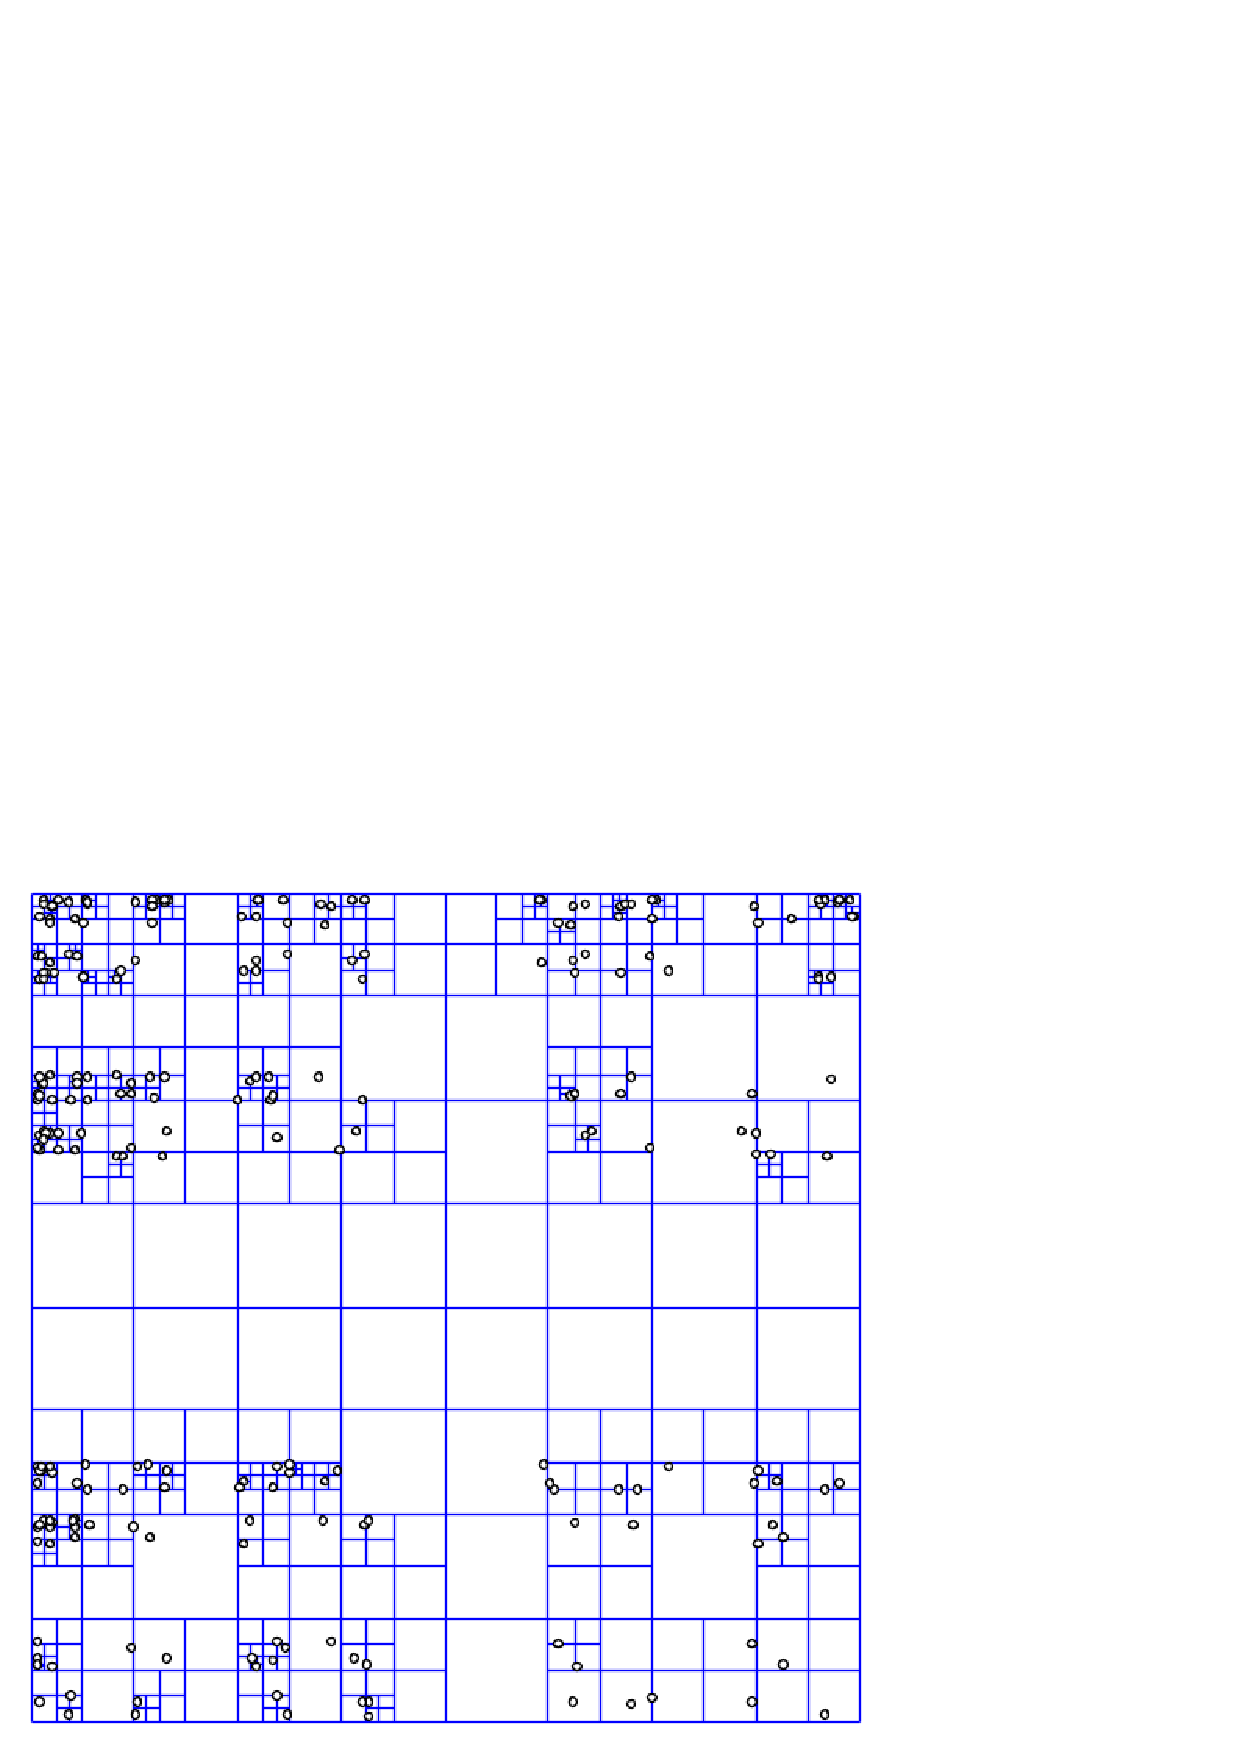
\includegraphics[scale=0.30]{quadtree}
\caption{Représentation d'un quadtree}
\end{figure}
Cette strucure pourrait être utilisé pour déterminer la position des boites dans l'espace selon la méthode suivante :
\begin{itemize}
\item Si un des nœuds du quadtree ne contient aucune boite ou qu'il est entièrement inclus dans un ensemble de boites alors il n'est plus nécessaire de le subdiviser. Ce nœud contiendra donc une référence sur chacune de ces boites.
\item \`A contrario si un nœud du quatree contient une des bornes d'une des boites, alors il est nécessaire de subdiviser ce nœud.
\item On arrête aussi de diviser les nœuds lorsque l'on arrive à une précision inférieur à la précision du calcul de Realpaver.
\end{itemize}
L'octree repose sur le même principe mais étendu à trois dimensions. L'espace est donc découpé en huit parties à chaque fois.

\paragraph{} Cette structure est particulièrement intéressante pour la visualisation du pavage. En effet pour une fenêtre de visualisation donnée, il est très simple et rapide d'extraire la sous-arborescence correspondante à l'espace visualisé et permet aussi de ne pas afficher les objets trop petits.

Le problème de cette méthode est essentiellement à la construction puisque la structure devra découper en la plus petite feuille possible au niveau des bornes des boites ce qui va nécessairement entrainer la construction d'un grand nombre de feuilles. Ce problème est particulièrement gênant puisque si l'on cherche à localiser une boite de dimensions 1 sur 1 avec la précision donnée par défaut par Realpaver de $10^{-16}$, on se retrouve avec au moins $4 \times 10^{16}$ feuilles. On peut optimiser l'algorithme de construction en considérant que si un des nœuds contient l'intégralité ou une partie d'une seule boite, il n'est plus nécessaire de subdiviser ; la recherche d'une seule boite étant immédiate.

Un autre problème
\end{document}
